%%%%%%%%%%%%%%%%%%%%%%%%%%%%%%%%%%%%%%%%%%%%%%%%%%%%%%%%%%%%%%%%%%%%%%%%%%%%%%%%
%
%
%
%%%%%%%%%%
\chapter{Umsetzung des RO-SLAM in ROS}
\label{ch:ro_slam}

Im vorherigen Kapitel wurden mehrere \gls{uwbm} erstellt, darunter befand sich ein \gls{tag} und vier \gls{anchor}. Um die Entfernungen messen zu können, muss der \gls{tag} auf einer Roboterplattform montiert und die \gls{anchor} im Messbereich verteilt werden. Damit ist aber nur ein Teil der Hardwareanforderungen erfüllt. Es wird noch eine Roboterplattform benötigt, die zum einen um den \gls{tag} erweitert werden kann und zum anderen über ausreichend Leistungsreserven verfügt um alle \glspl{rosm} ausführen zu können, die für einen \gls{roslam} benötigt werden. Die Zusammenstellung dieser Roboterplattform ist bestandteil dieses Kapitel.

Die eingesetze Hardware bildet einen soliden Sockel für die Ausführung der \glspl{rosm}. Erweitert werden muss dieser noch um die Softwareseite. Mit der Übersicht über die Softwarearchitektur lässt sich eine grobe Vorstellung der eingesetzten \glspl{rosm} vermitteln. Einen tieferen Einblick in die \glspl{rosm} liefern die Abschnitte mit den \gls{ros}-Hauptmodulen und -Nebenmodulen. Bei dem ersteren geht es um die Kernmodule die eine direkte bzw. indirekte Voraussetzung für den \gls{roslam} sind. Im letzteren werden die Module behandeln die notwendigen sind um zusätzliche Daten, Kennzahlen und Grafiken für die Auswertung zu extrahieren.

Nach dem die Hardware- und Softwarevoraussetzungen für den \gls{roslam} Algorithmus erfüllt wurden, wird ein Blick auf die Umsetzung des \gls{roslam} in dem \gls{mrpt}-Framework geworfen.


%%%%%%%%%%%%%%%%%%%%%%%%%%%%%%%%%%%%%%%%%%%%%%%%%%%%%%%%%%%%%%%%%%%%%%%%%%%%%%%%
%
%	- Einsatz mobiler Roboter in der Logistik am Beispiel des Robotino
%		- http://www.r-moehrle.de/wissenschaftlicheArbeiten/robotino1.pdf
%
%%%%%%%%%%
\section{Roboterplattform}

Um die Messungen für den \Gls{roslam} aufzuzeichnen wird eine Roboterplattform benötigt, auf der das \Gls{uwbm} montiert werden kann. Zusätzlich wird noch eine Reihe weiterer Sensoren benötigt, die im Folgenden vorgestellt werden.

Also Roboterplattform dient dabei der Robotino 2 von \textit{Festo Didactic}. Er gehört zur Klasse der holonomen Roboter, d.h. seinen Bewegungsmöglichkeiten unterliegen keinerlei Einschränkungen im zweidimensionalen Raum. Ermöglicht wird das, durch drei voneinander unabhängig arbeitenden omnidirektionalen Antriebseinheiten. Jede der drei Antriebseinheiten verfügt über einen Inkrementalgeber, mit dessen Hilfe abgeschätz wird, wie weit der Robotino gefahren ist. Um den Fehler der Inkrementalgeber in Kurvenfahrten zu reduzieren wird das digitale Gyroskop\footnotemark{} von \textit{Microinfinity} eingesetzt. Gesteuert wird der Robotino über eine \SI{300}{\MHz} starke Verarbeitungseinheit auf Basis eines Linux Betriebssystems mit einem Echtzeitkernel. \cite{festo2007robotinomanual} \footnotetext{Model: CruizCore XG1000 / XG1010}

An der höchsten Position des Robotinos befindet sich ein 2D-Laser-Entfernungsmesser\footnotemark{} der Firma \textit{Sick}. Mit einem Öffnungswinkel von \SI{270}{\degree} und einem Arbeitsbereich von \SIrange{0.05}{25}{\meter} ist es möglich, genaue Belegtheitskarten der Umwelt zu erstellen. \cite{sick2016operatingmanual} \footnotetext{Model: TiM571-2050101}

Die Verarbeitungseinheit des Robotinos ist leistungsfähig genug um die anstehenden Steuerungsaufgaben zu erfüllen. Jedoch ist diese von leistungshungrigen Anwendungen wie dem \Gls{roslam} überfordert. Aus diesem Grund wird eine zusätzliche Verarbeitungseinheit\footnote{Model: NUC5i7RYH} mit einem Intel Core i7\footnote{5. Generation des Intel Core i7-5557U Prozessor mit bis zu \SI{3.4}{\GHz}. \cite{intel2015nucproductbrief}} verwendet.

Die Fahrbefehle werden dem Robotino über einen Xbox Wireless Controller übermittelt.

\begin{figure}
	\centering
	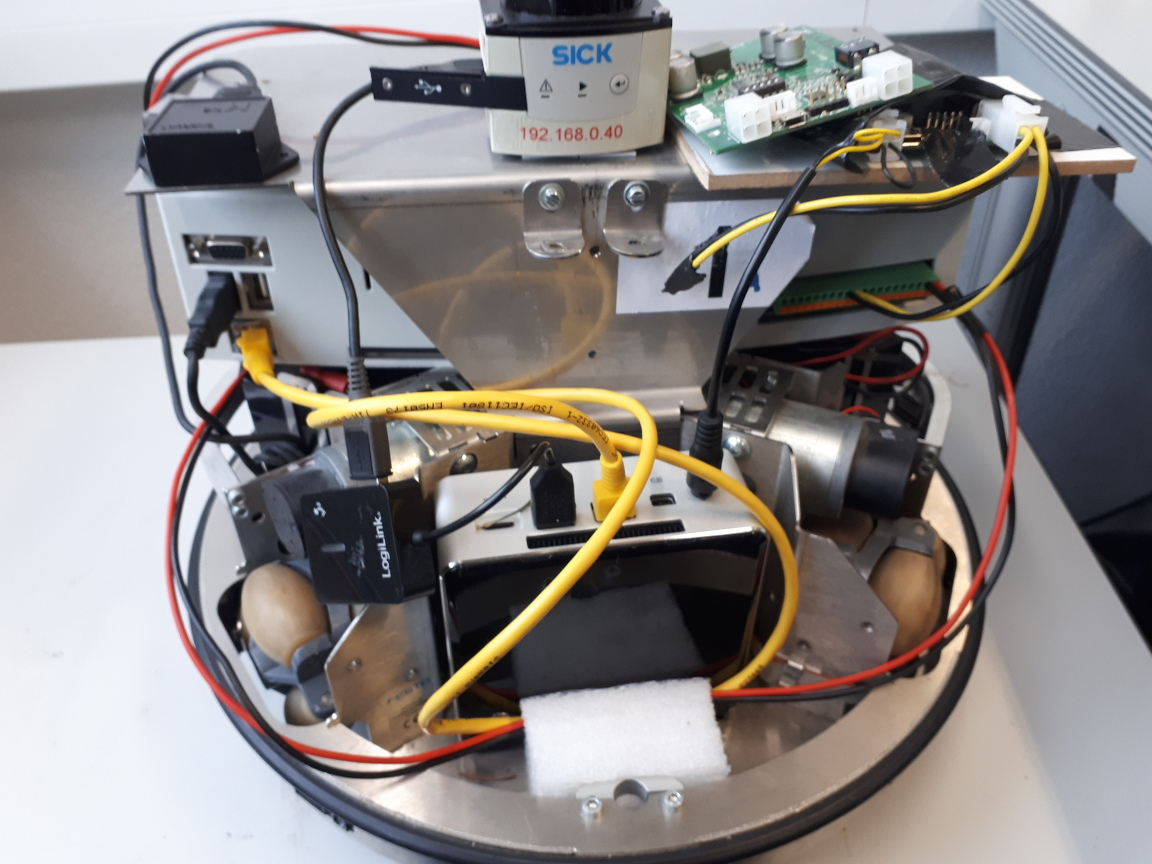
\includegraphics[width=0.5\textwidth]{robotino_front}
	\caption{Frontansicht der fertig aufgebauten Roboterplattform.}
	\label{fig:robotino_front}
\end{figure}
% todo: Professionelleres Foto verwenden.


%%%%%%%%%%%%%%%%%%%%%%%%%%%%%%%%%%%%%%%%%%%%%%%%%%%%%%%%%%%%%%%%%%%%%%%%%%%%%%%%
%
%	- Kurzbeschreibung der Modulfunktion
%	- Welche Funktion erfüllt dieses Modul
%	- Welche ROS-Messages/-Topics/-Services bietet dieses Modul
%
%%%%%%%%%%
\section{Softwarearchitektur}

Der Softwarearchitektur, siehe \autoref{fig:architektur_grouped}, lassen sich zwei Nachrichtentypen entnehmen die für den \gls{roslam} essentiell sind. Zum einen sind das die Daten der Entfernungsmessungen (\textit{mrpt\_msgs/ObservationRangeBeacon}) zwischen den \gls{uwbm} und dem Transformationsbaum (\textit{tf2\_msgs/TFMessage}) auf der anderen. Die Nachrichten des Transformationsbaums werden dabei nur indirekt benötigt, um zu bestimmen wie weit sich die Roboterplattform bewegt hat, sprich die Odometrieinformationen.

Als Datenquelle für den Transformationsbaum sind zuerst die statischen Transformationen zu nennen, dann die Belegtheitskarten für die Transformation von dem Odometrie- in das Kartenkoordinatensystem und zuletzt die zwei Arten der Odometrie. Die erste liefert die Daten anhand der Inkrementalgeber in der Antriebseinheit und die zweite eine Odometrie über das auswerten der 2D-Laser-Entfernungsmessers. Bei der Laser-Odometrie haben sich zwei unterschiedliche Verfahren etabliert und alle drei Verfahren sollen auf ihre Genauigkeit Untersucht werden.

Der untere Bereich ist über keinen Datenbus mit den anderen \gls{rosm} verbunden. Jedoch wird dieser zum einen benötigt um die Kommunikation zwischen der Robotino Steuereinheit herzustellen und zum anderem um die Roboterplattform als Ganzes durch ein Eingabegerät zu steuern.

\begin{figure}
	\centering
	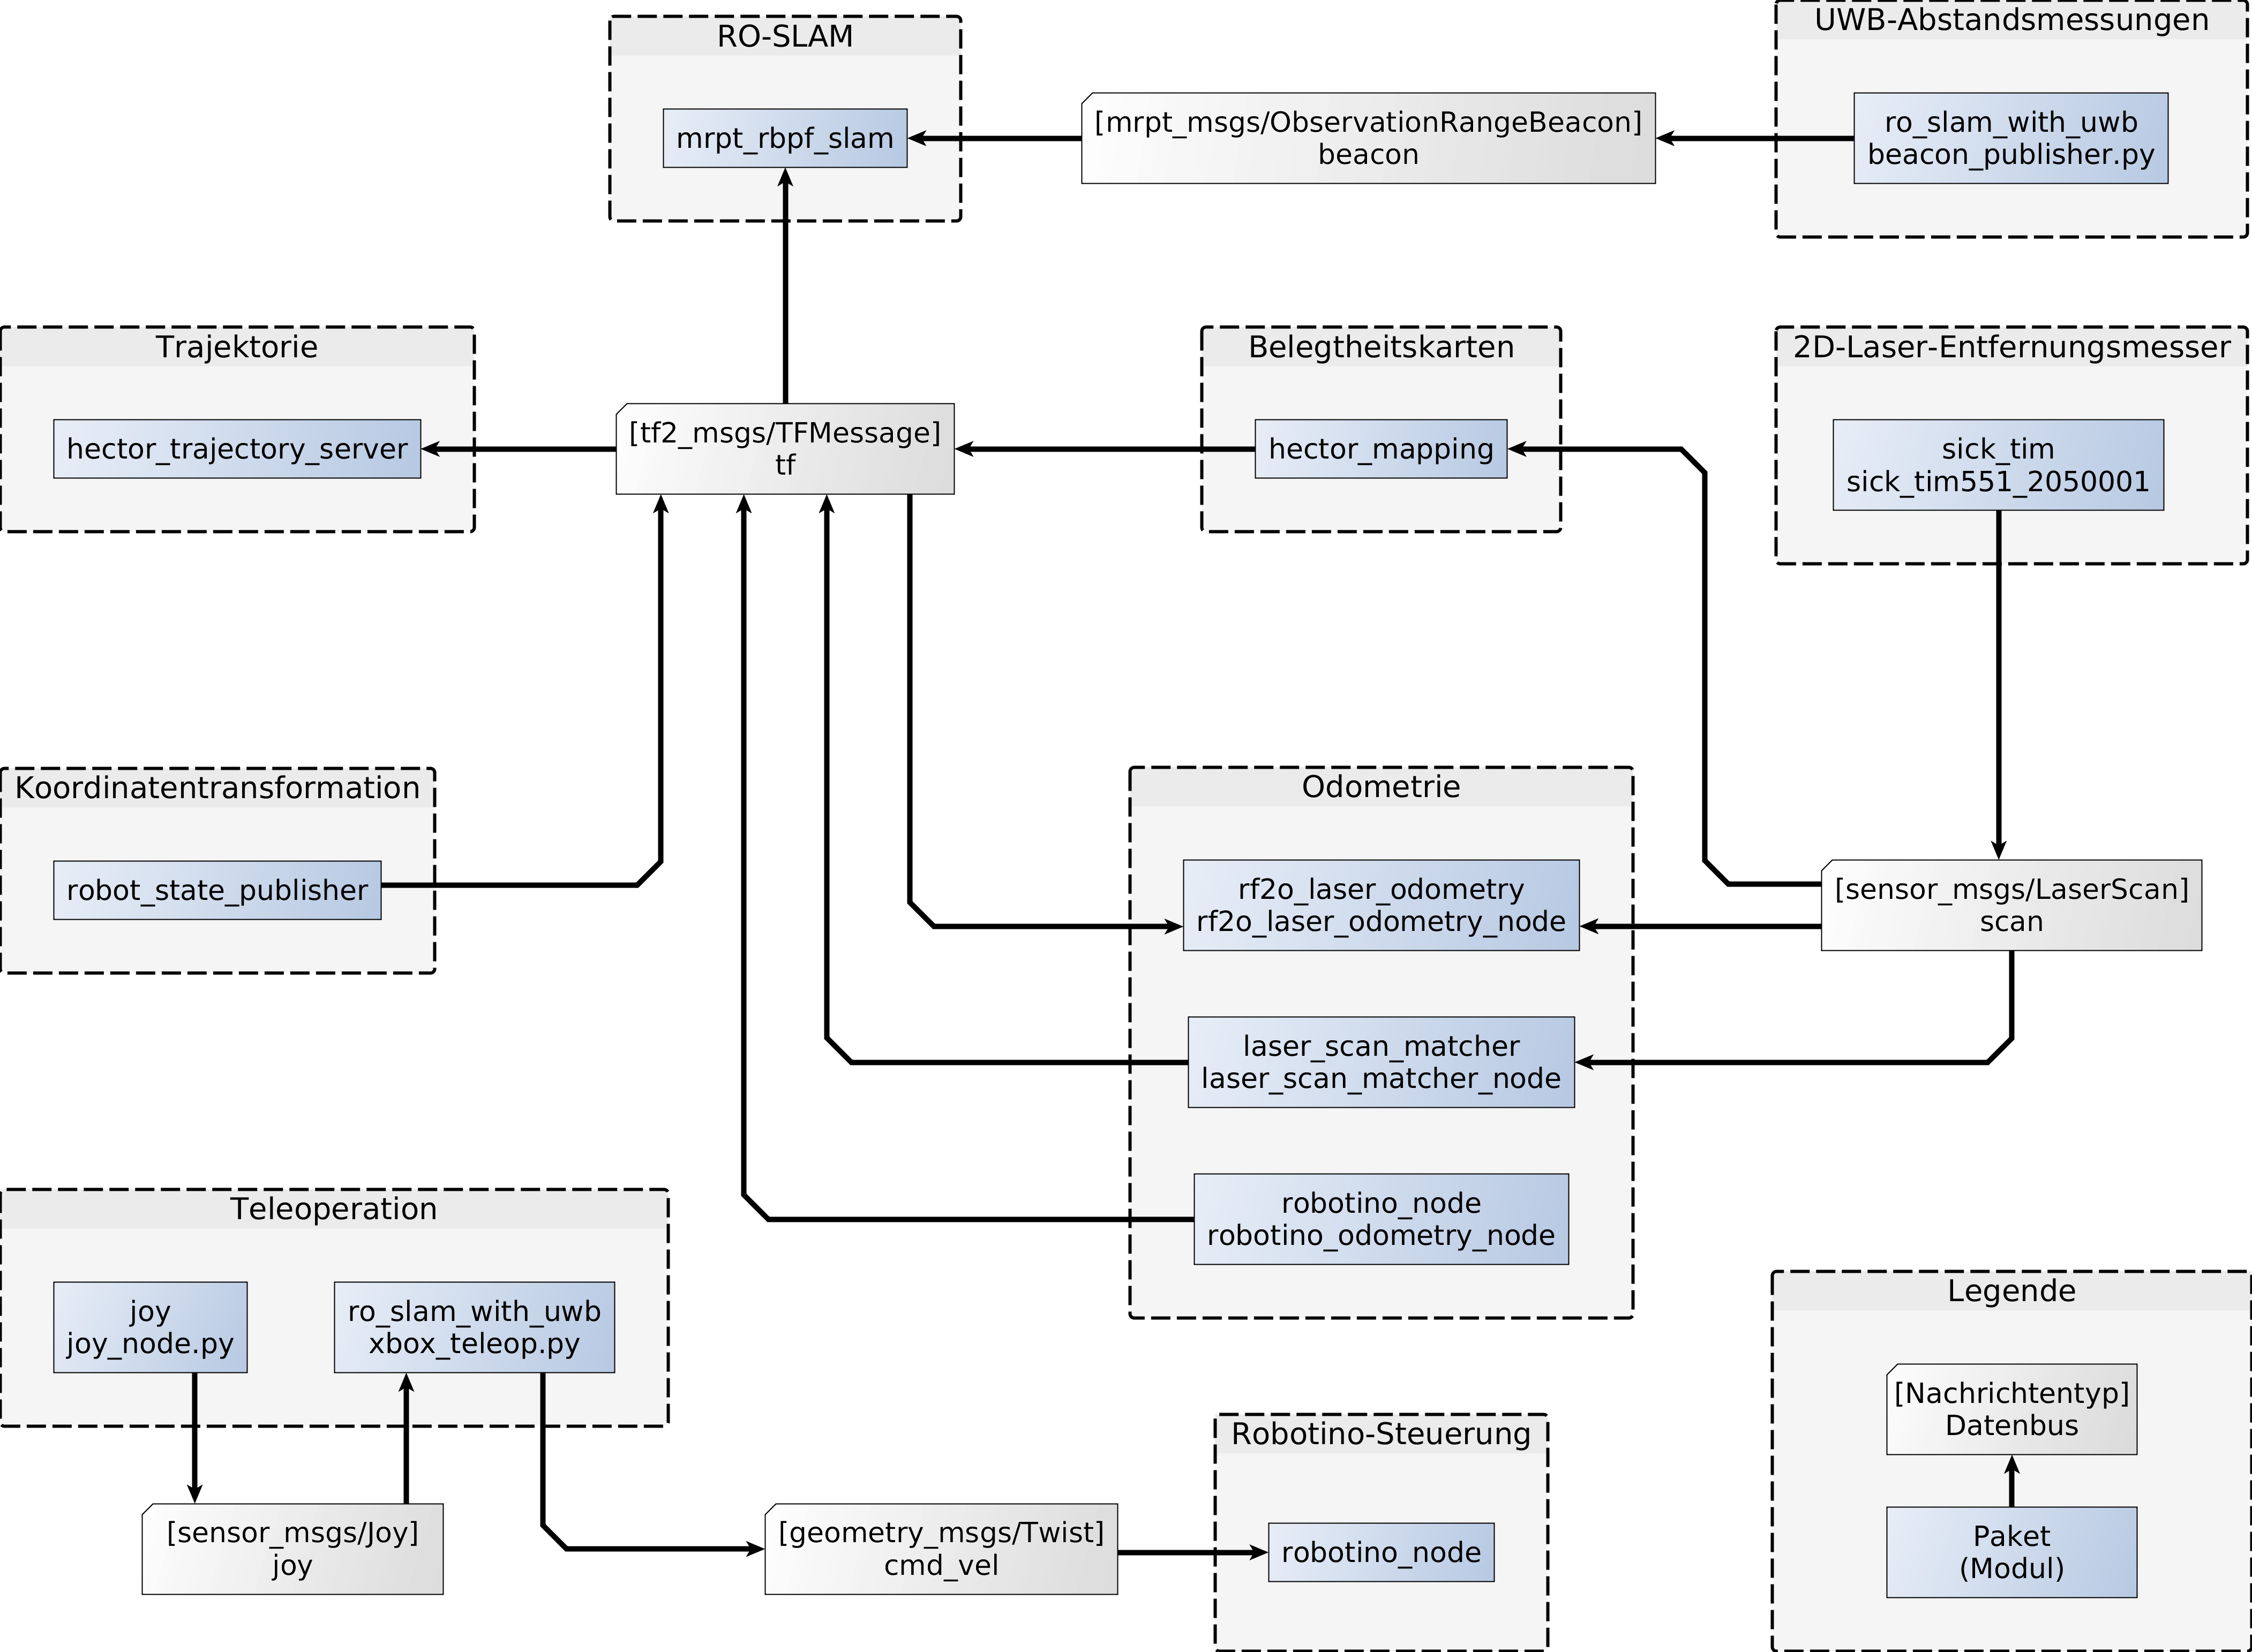
\includegraphics[width=\linewidth]{architektur_grouped}
	\caption{Softwarearchitektur der \glspl{rosm} für den \glsentryshort{roslam}.}
	\label{fig:architektur_grouped}
\end{figure}


%%%%%%%%%%%%%%%%%%%%%%%%%%%%%%%%%%%%%%%%%%%%%%%%%%%%%%%%%%%%%%%%%%%%%%%%%%%%%%%%
%
%
%
%%%%%%%%%%
\subsection{ROS-Hauptmodule}


%%%%%%%%%%%%%%%%%%%%%%%%%%%%%%%%%%%%%%%%%%%%%%%%%%%%%%%%%%%%%%%%%%%%%%%%%%%%%%%%
%
%	- \url{http://wiki.ros.org/robotino_node}
%	- Service reset_odometry
%
%%%%%%%%%%
\subsubsection{Robotino-Steuerung}

Zur Steuerung der Roboterplattform muss die Verarbeitungseinheit Befehle zur Steuereinheit des Robotinos schicken. Diese Aufgabe erfüllt das \Gls{rosm} \textit{robotino\_node} aus dem Paket \textit{robotino\_node}. Über den Datenbus \textit{cmd\_vel} können die Geschwindigkeiten in X-/Y-Richtung und um die Z-Achse festgelegt werden. Um den Robotino zu stoppen, müssen alle drei Parameter auf den Wert null gesetzt werden.

Um an die Informationen der Inkrementalgeber zu kommen, muss das \Gls{rosm} \textit{robotino\_odometry\_node} aus dem Paket \textit{robotino\_node} gestartet werden. Nach dem Start steht der Datenbus \textit{odom} mit den aktuellen Werte der Inkrementalgeber zur Verfügung. Zusätzlich sorgt dieses Modul auch für die dynamische Transformation zwischen dem \textit{odom} und \textit{base\_link} Koordinatensystem.


%%%%%%%%%%%%%%%%%%%%%%%%%%%%%%%%%%%%%%%%%%%%%%%%%%%%%%%%%%%%%%%%%%%%%%%%%%%%%%%%
%
%	- \url{http://wiki.ros.org/robot_state_publisher}
%	- \url{http://wiki.ros.org/urdf}
%
%%%%%%%%%%
\subsubsection{Koordinatentransformation}

Neben den dynamischen Transformationen besteht die Roboterplattform auch aus vielen statischen Transformationen. Hierzu gehört z.B. die Transformation vom Mittelpunkt der Roboterplattform zum 2D-Laser-Entfernungsmesser oder \Gls{uwbm}. Diese statischen Transformationen werden in einer \Gls{urdf}-Datei einmalig gespeichert und dann über das \Gls{rosm} \textit{state\_publisher} aus dem Paket \textit{robot\_state\_publisher} zur Laufzeit bereitgestellt, siehe \autoref{fig:rviz_robotino_tf2}.

\begin{figure}
	\centering
	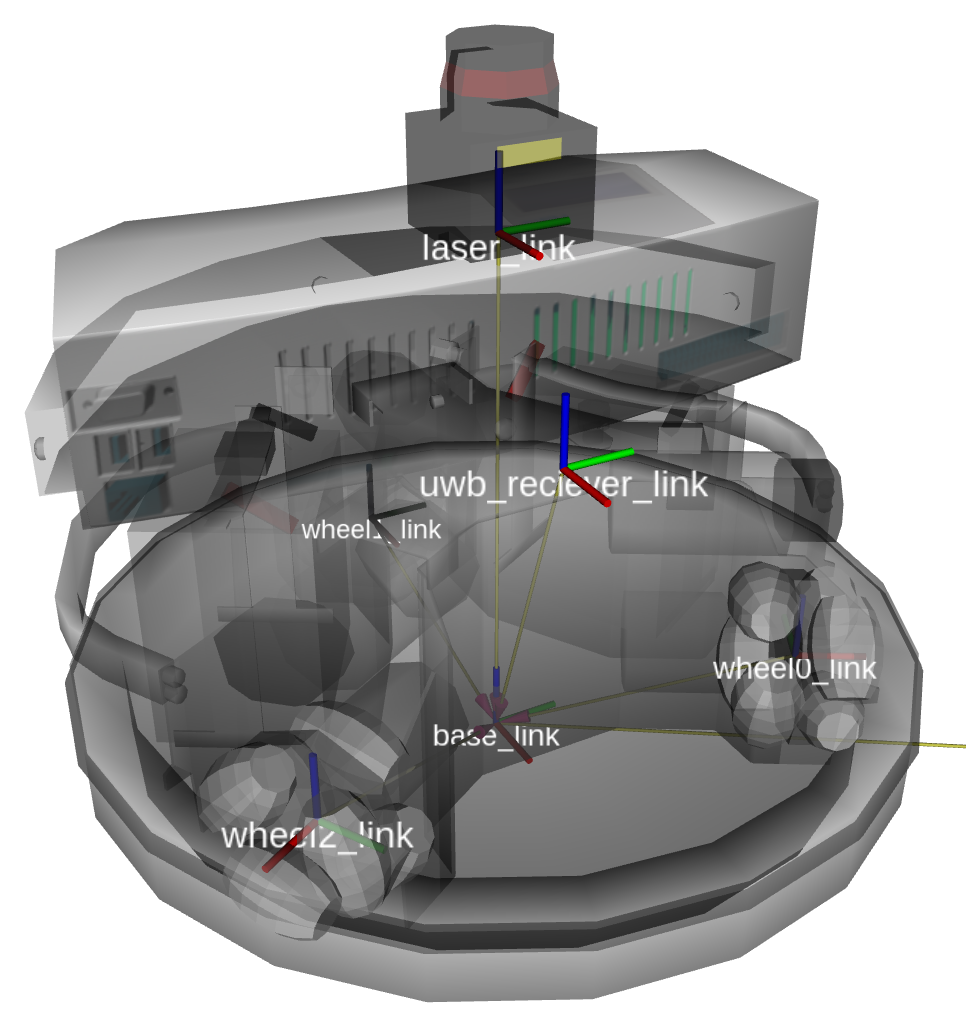
\includegraphics[width=0.5\linewidth]{rviz_robotino_tf2}
	\caption{Statische Transformationen der Roboterplattform.}
	\label{fig:rviz_robotino_tf2}
\end{figure}


%%%%%%%%%%%%%%%%%%%%%%%%%%%%%%%%%%%%%%%%%%%%%%%%%%%%%%%%%%%%%%%%%%%%%%%%%%%%%%%%
%
%	- \url{http://wiki.ros.org/joy}
%
%%%%%%%%%%
\subsubsection{Teleoperation}

Zur Steuerung der Roboterplattform wird ein \textit{Xbox Wireless Controller} als Eingabegerät verwendet. Zustandsänderungen werden über das \Gls{rosm} \textit{joy\_node} aus dem Paket \textit{joy} registriert und über den Datenbus \textit{joy} bereitgestellt. Das überwachte Eingabegerät wird über den Parameter \textit{dev} festgelegt.
%, siehe \autoref{lst:joy_node}.

Mit den generischen Daten des Eingabegerätes kann die Roboterplattform nichts anfangen, diese benötigt eine Nachricht vom Typ \textit{geometry\_msgs/Twist}. Die Transformation zwischen der Nachricht \textit{sensor\_msgs/Joy} und \textit{geometry\_msgs/Twist} erfolgt durch das \Gls{rosm} \textit{xbox\_teleop.py} aus dem Paket \textit{ro\_slam\_with\_uwb}.


%%%%%%%%%%%%%%%%%%%%%%%%%%%%%%%%%%%%%%%%%%%%%%%%%%%%%%%%%%%%%%%%%%%%%%%%%%%%%%%%
%
%
%
%%%%%%%%%%
\subsubsection{UWB-Entfernungsmessung}

Die Entfernungsmessung zwischen dem \Gls{tag} und den vorhandenen \Glspl{anchor} werden durch das \Gls{uwbm} über die \Gls{usb}-Schnittstelle bereitgestellt. Die Daten werden dann von dem \Gls{rosm} \textit{beacon\_publisher.py} aus dem Paket \textit{ro\_slam\_with\_uwb} aufgefangen und auf den Datenbussen \textit{beacon} und \textit{beacon\_raw} veröffentlicht. Der erste Datenbus ist vom Typ \textit{mrpt\_msgs/ObservationRangeBeacon} und wird von dem \Gls{mrpt}-Modul für den \Gls{roslam} benötigt. Der zweite Datenbus wird für die Auswertung der Entfernungsmessung im \autoref{ch:eval} benötigt und ist vom Typ \textit{ro\_slam\_with\_uwb/Beacon}.


%%%%%%%%%%%%%%%%%%%%%%%%%%%%%%%%%%%%%%%%%%%%%%%%%%%%%%%%%%%%%%%%%%%%%%%%%%%%%%%%
%
%
%
%%%%%%%%%%
\subsection{ROS-Hilfsmodule}


%%%%%%%%%%%%%%%%%%%%%%%%%%%%%%%%%%%%%%%%%%%%%%%%%%%%%%%%%%%%%%%%%%%%%%%%%%%%%%%%
%
%	- \url{http://wiki.ros.org/sick_tim}
%
%%%%%%%%%%
\subsubsection{2D-Laser-Entfernungsmesser}

Der 2D-Laser-Entfernungsmesser gehört zu einem der am häufigsten verwendeten Sensoren für die präzise visuelle Erfassen der Umwelt. Für mehrere der nachfolgenden \Gls{rosm} ist eine 2D-Laser-Entfernungsmessung eine zwingende Voraussetzung. Um die Daten dem \Gls{ros}-System bereitzustellen wird das \Gls{rosm} \textit{sick\_tim551\_2050001} aus dem Paket \textit{sick\_tim} verwendet. Dieses Modul stellt über den Datenbus \textit{scan}, mit einer Rate von \SI{15}{\hertz}, Nachrichten vom Typ \textit{sensor\_msgs/LaserScan} bereit.


%%%%%%%%%%%%%%%%%%%%%%%%%%%%%%%%%%%%%%%%%%%%%%%%%%%%%%%%%%%%%%%%%%%%%%%%%%%%%%%%
%
%	- \url{http://wiki.ros.org/hector_mapping}
%
%%%%%%%%%%
\subsubsection{Belegtheitskarten}

Das erste \Gls{rosm}, das von der 2D-Laser-Entfernungsmessung Gebrauch macht, ist das \textit{hector\_mapping} aus dem Paket \textit{hector\_mapping}. Mit diesem Modul können präzise Belegtheitskarten (engl. Occupancy Grid Map) erstellt werden, die für jede Koordinate der Karte festlegen ob diese durch ein Hindernis belegt (schwarz) oder frei (weiß) ist. Bereiche die von Hindernissen verdeckt sind oder außerhalb der Sensorreichweite liegen, werden als unbestimmt (grau) markiert, siehe \autoref{fig:rviz_occupancy_grid_map}. In \Gls{ros} werden Belegtheitskarten mit dem Nachrichtentyp \textit{nav\_msgs/OccupancyGrid} repräsentiert.

Über die minimale und maximale Sensorreichweite (\textit{laser\_min\_dist} bzw. \textit{laser\_max\_dist}) wird festgelegt, welche Messungen für die Kartenerstellung berücksichtigt werden. Es ist sinnvoll die Herstellerangaben von \SI{0.05}{\meter} und \SI{25.0}{\meter} zu verwenden.

Die Auflösung einer Zelle in der Karte wird über den Parameter (\textit{map\_resolution}) festgelegt. Es eine Auflösung von \SI{0.02}{\meter} pro Zelle verwendet.

\begin{figure}
	\centering
	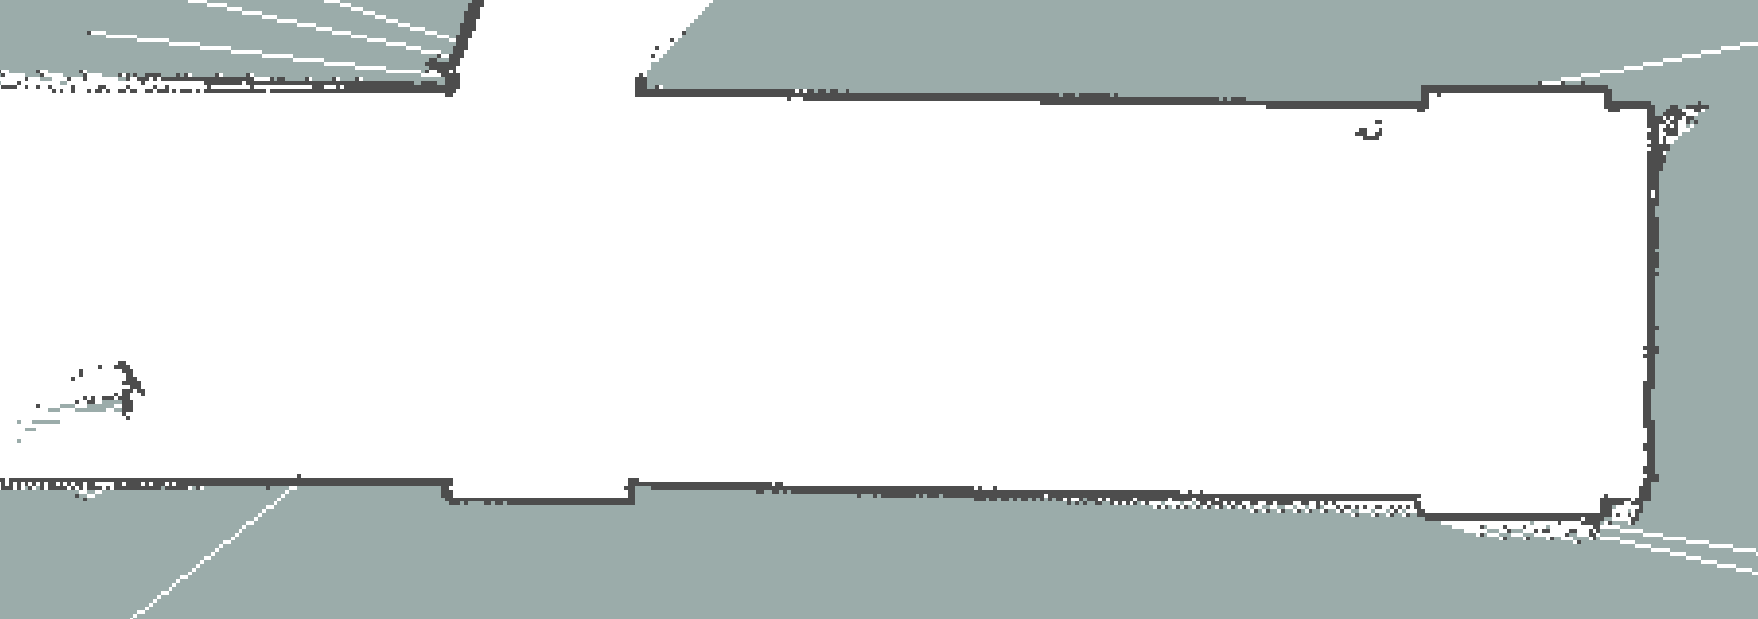
\includegraphics[width=0.9\linewidth]{rviz_occupancy_grid_map}
	\caption{Die Belegtheitskarte der Messstrecke.}
	\label{fig:rviz_occupancy_grid_map}
\end{figure}
 

%%%%%%%%%%%%%%%%%%%%%%%%%%%%%%%%%%%%%%%%%%%%%%%%%%%%%%%%%%%%%%%%%%%%%%%%%%%%%%%%
%
%	- \url{http://wiki.ros.org/hector_trajectory_server}
%	- \url{http://docs.ros.org/api/nav_msgs/html/msg/Path.html}
%
%%%%%%%%%%
\subsubsection{Trajektorie}

Neben den Entfernungsinformationen wertet der \Gls{roslam} auch die Daten der Odometrie aus. Als Quelle für die Odometrie dienen dabei die Inkrementalgeber der Robotorplattform. Im nächsten Abschnitt werden weitere Quellen für die Odometrie vorgestellt. Um die Güte der Odometrie-Quellen zu vergleichen, wird die verfahrene Trajektorie jeder Quelle benötigt. Diese Informationen werden von dem \Gls{rosm} \textit{hector\_trajectory\_server} aus dem Paket {hector\_trajectory\_server} bereitgestellt. Die Daten liegen dabei als Nachricht vom Typ \textit{nav\_msgs/Path} bereit und können in die Belegtheitskarte integriert werden, siehe \autoref{fig:rviz_trajektorie}.

\begin{figure}
	\centering
	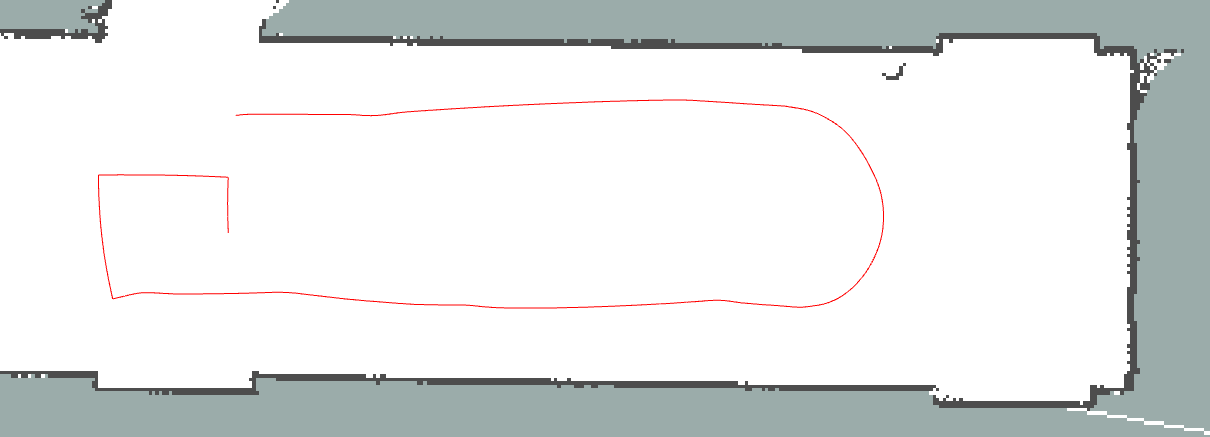
\includegraphics[width=0.9\linewidth]{rviz_trajektorie}
	\caption{Die Trajektorie einer Messfahrt der Roboterplattform.}
	\label{fig:rviz_trajektorie}
\end{figure}


%%%%%%%%%%%%%%%%%%%%%%%%%%%%%%%%%%%%%%%%%%%%%%%%%%%%%%%%%%%%%%%%%%%%%%%%%%%%%%%%
%
%	- \url{http://wiki.ros.org/rf2o}
%	- \url{http://wiki.ros.org/laser_scan_matcher}
%
%%%%%%%%%%
\subsubsection{Laser-Odometrie}

Wie bereits im vorherigen Abschnitt erwähnt, werden hier zwei weitere Quelle für die Odometrie vorgestellt. Beide \Glspl{rosm} nutzen nur die Daten der 2D-Laser-Entfernungsmessung um eine Schätzung für die aktuelle Pose zu erstellen.

Bei dem ersten \gls{rosm} handelt es sich um den \textit{laser\_scan\_matcher\_node} aus dem Paket \textit{laser\_scan\_matcher}. Hierbei handelt es sich um eine Variante des \gls{icp}-Verfahrens, welches versucht eine Transformation zwischen den Punkt einer Oberfläche aus den vorherigen und aktuellen Sensordaten zu finden. Jedoch wird anstatt einer Punkt-zu-Punkt- eine Punkt-zu-Linie-Metrik für die Minimierung verwendet. \cite{censi2008icp} Dieses Verfahren wird im Folgenden nur noch als LSM-Verfahren bezeichnet.

Bei dem zweiten \gls{rosm} handelt es sich um den \textit{rf2o\_laser\_odometry\_node} aus dem Paket \textit{rf2o\_laser\_odometry}. Hierbei handelt es sich um eine Implementierung des \gls{rf2o}-Verfahrens, bei dem jeder beobachtete Punkt des Sensors als eine Funktion der Geschwindigkeit des Sensors modelliert wird. Die Bewegung des Sensors wird dann aus der Minimierung der Dichteformulierung aller Punkt-Funktionen berechnet. \cite{jaimez2016planar}


%%%%%%%%%%%%%%%%%%%%%%%%%%%%%%%%%%%%%%%%%%%%%%%%%%%%%%%%%%%%%%%%%%%%%%%%%%%%%%%%
%
%	- \url{https://www.mrpt.org}
%	- \url{http://wiki.ros.org/mrpt_slam}
%	- \url{http://wiki.ros.org/mrpt_navigation}
%	- \url{https://www.mrpt.org/tutorials/slam-algorithms/rangeonly_slam/}
%		- Bayesian range-only SLAM (RO-SLAM) with SOGs
%	- \url{http://mrpt.ual.es/reference/devel/classmrpt_1_1slam_1_1_c_metric_map_builder_r_b_p_f.html}
%		- mrpt::slam::CMetricMapBuilderRBPF Class Reference
%		- It is actually a front-end to the class mrpt::slam::CMetricMapBuilderRBPF.
%		- All the parameters to the algorithm are passed through a configuration file in the command line.
%		- The filter processes actions and observations from a rawlog file and optionally generates a number of files describing the evolution of the filter and the maps.
%
%%%%%%%%%%
\subsection{MRPT}

Bei dem \Gls{mrpt}-Framework handelt es sich um eine Bibliothek die Datenstrukturen und Algorithmen aus dem aktiven Forschungsbereich der Robotik bereitstellt. Dadurch ist eine schnelle Umsetzung neuer Algorithmen, sowie der Vergleich mit bereits bestehenden möglich. Zu den verfügbaren Datenstrukturen zählen die Basisdatentypen der linearen Algebra bis hin zu den komplexeren Datentypen der Robotik wie z.B. die Belegtheitskarten. Zur direkten Verwendung existieren viele Algorithmen aus den Bereichen der \Gls{slam}-Algorithmen, des Maschinellen Sehen (engl. Computer Vision) und der Pfad- und Bewegungsplanung (engl. Path/Motion Planning).

Aus dem Bereich der \Gls{roslam}-Algorithmen sind die Verfahren aus den Veröffentlichungen \citetitle{blanco2008pure} und \citetitle{blanco2008efficient} implementiert, siehe \autoref{sec:blanco2008pure} und \ref{sec:blanco2008efficient}.

Um die \Gls{roslam}-Algorithmen aus dem \Gls{mrpt}-Framework zu nutzen, wird das \Gls{rosm} \textit{mrpt\_rbpf\_slam} aus dem Paket \textit{mrpt\_rbpf\_slam} benötigt. Mit dem Parameter \textit{ini\_filename} wird der Dateipfad zu der Konfigurationdatei für die \Gls{roslam}-Algorithmen angegeben und über den \textit{sensor\_source} Parameter werden die Datenquellen für den \Gls{roslam} definiert. Hierbei ist es möglich sowohl die Entfernungsmessungen der \Gls{uwbm} als auch die der 2D-Laser-Entfernungsmesser anzugeben. Von der letzten Datenquelle wird kein gebraucht gemacht, da dadurch Transformationen zwischen Koordinatensystemen veröffentlicht werden die mit den bereits bestehenden kollidieren. Über die Datenbusse \textit{particlecloud} und \textit{particlecloud\_beacons} werden die Positionsschätzungen für die Roboterplattform und die \Glspl{uwbm} veröffentlicht, siehe \autoref{fig:rviz_robot_and_beacon_estimate}.

\begin{figure}
	\centering
	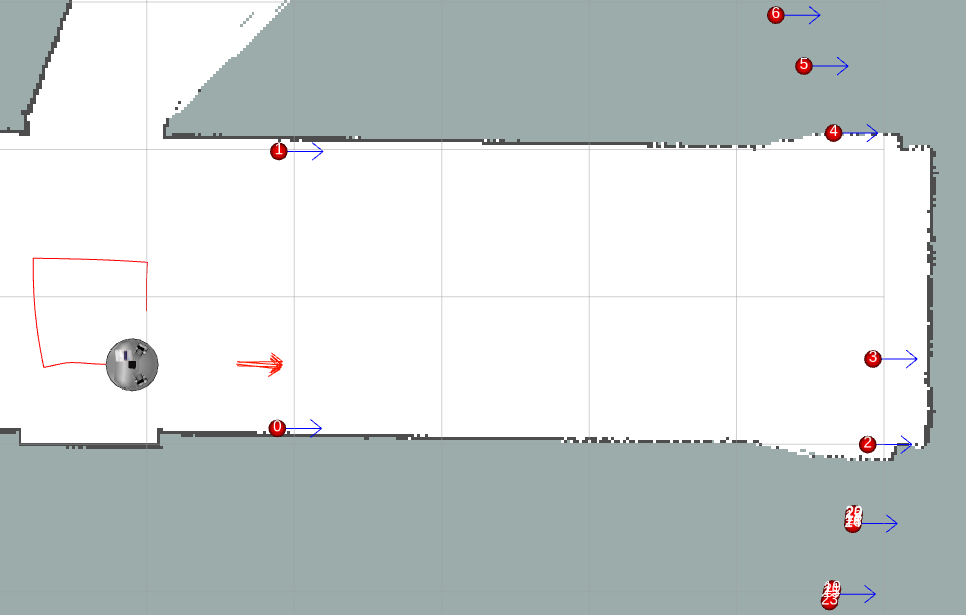
\includegraphics[width=0.9\linewidth]{rviz_robot_and_beacon_estimate}
	\caption{Positionsschätzung für die Roboterplattform mit roten Pfeilen und für die \Glspl{uwbm} mit blauen Pfeilen.}
	\label{fig:rviz_robot_and_beacon_estimate}
\end{figure}

Nach der Konfiguration der \Gls{ros} Seite müssen noch Einstellungen für den \Gls{roslam} festgelegt werden. Hier muss die Konfigurationsdatei, die in dem \Gls{ros}-Parameter \textit{ini\_filename} hinterlegt ist, bearbeitet werden. Das \Gls{mrpt}-Framework verfügt über einen eigenen Abspielmechanismus für aufgezeichnete Messungen. Dieser wird nicht verwendet, da \Gls{ros} über einen eigenen Mechanismus verfügt. Folglich wird der Parameter \textit{rawlog\_file=} auf einen leeren Wert gesetzt werden. Auch verfügt \Gls{ros} über eine eigene Visualisierungslösung, daher wird die grafische Anzeige des \Gls{mrpt}-Frameworks über den Parameter \textit{SHOW\_PROGRESS\_IN\_WINDOW=0} deaktiviert. Um zwischen den beiden \Gls{roslam}-Verfahren zu wechseln, wird der Parameter \textit{insertAsMonteCarlo} angepasst werden.

